% Options for packages loaded elsewhere
\PassOptionsToPackage{unicode}{hyperref}
\PassOptionsToPackage{hyphens}{url}
%
\documentclass[
]{article}
\usepackage{lmodern}
\usepackage{amssymb,amsmath}
\usepackage{ifxetex,ifluatex}
\ifnum 0\ifxetex 1\fi\ifluatex 1\fi=0 % if pdftex
  \usepackage[T1]{fontenc}
  \usepackage[utf8]{inputenc}
  \usepackage{textcomp} % provide euro and other symbols
\else % if luatex or xetex
  \usepackage{unicode-math}
  \defaultfontfeatures{Scale=MatchLowercase}
  \defaultfontfeatures[\rmfamily]{Ligatures=TeX,Scale=1}
\fi
% Use upquote if available, for straight quotes in verbatim environments
\IfFileExists{upquote.sty}{\usepackage{upquote}}{}
\IfFileExists{microtype.sty}{% use microtype if available
  \usepackage[]{microtype}
  \UseMicrotypeSet[protrusion]{basicmath} % disable protrusion for tt fonts
}{}
\makeatletter
\@ifundefined{KOMAClassName}{% if non-KOMA class
  \IfFileExists{parskip.sty}{%
    \usepackage{parskip}
  }{% else
    \setlength{\parindent}{0pt}
    \setlength{\parskip}{6pt plus 2pt minus 1pt}}
}{% if KOMA class
  \KOMAoptions{parskip=half}}
\makeatother
\usepackage{xcolor}
\IfFileExists{xurl.sty}{\usepackage{xurl}}{} % add URL line breaks if available
\IfFileExists{bookmark.sty}{\usepackage{bookmark}}{\usepackage{hyperref}}
\hypersetup{
  pdftitle={A születésszám és a gazdaság kapcsolata},
  pdfauthor={Granát Marcell},
  hidelinks,
  pdfcreator={LaTeX via pandoc}}
\urlstyle{same} % disable monospaced font for URLs
\usepackage[margin=1in]{geometry}
\usepackage{color}
\usepackage{fancyvrb}
\newcommand{\VerbBar}{|}
\newcommand{\VERB}{\Verb[commandchars=\\\{\}]}
\DefineVerbatimEnvironment{Highlighting}{Verbatim}{commandchars=\\\{\}}
% Add ',fontsize=\small' for more characters per line
\usepackage{framed}
\definecolor{shadecolor}{RGB}{248,248,248}
\newenvironment{Shaded}{\begin{snugshade}}{\end{snugshade}}
\newcommand{\AlertTok}[1]{\textcolor[rgb]{0.94,0.16,0.16}{#1}}
\newcommand{\AnnotationTok}[1]{\textcolor[rgb]{0.56,0.35,0.01}{\textbf{\textit{#1}}}}
\newcommand{\AttributeTok}[1]{\textcolor[rgb]{0.77,0.63,0.00}{#1}}
\newcommand{\BaseNTok}[1]{\textcolor[rgb]{0.00,0.00,0.81}{#1}}
\newcommand{\BuiltInTok}[1]{#1}
\newcommand{\CharTok}[1]{\textcolor[rgb]{0.31,0.60,0.02}{#1}}
\newcommand{\CommentTok}[1]{\textcolor[rgb]{0.56,0.35,0.01}{\textit{#1}}}
\newcommand{\CommentVarTok}[1]{\textcolor[rgb]{0.56,0.35,0.01}{\textbf{\textit{#1}}}}
\newcommand{\ConstantTok}[1]{\textcolor[rgb]{0.00,0.00,0.00}{#1}}
\newcommand{\ControlFlowTok}[1]{\textcolor[rgb]{0.13,0.29,0.53}{\textbf{#1}}}
\newcommand{\DataTypeTok}[1]{\textcolor[rgb]{0.13,0.29,0.53}{#1}}
\newcommand{\DecValTok}[1]{\textcolor[rgb]{0.00,0.00,0.81}{#1}}
\newcommand{\DocumentationTok}[1]{\textcolor[rgb]{0.56,0.35,0.01}{\textbf{\textit{#1}}}}
\newcommand{\ErrorTok}[1]{\textcolor[rgb]{0.64,0.00,0.00}{\textbf{#1}}}
\newcommand{\ExtensionTok}[1]{#1}
\newcommand{\FloatTok}[1]{\textcolor[rgb]{0.00,0.00,0.81}{#1}}
\newcommand{\FunctionTok}[1]{\textcolor[rgb]{0.00,0.00,0.00}{#1}}
\newcommand{\ImportTok}[1]{#1}
\newcommand{\InformationTok}[1]{\textcolor[rgb]{0.56,0.35,0.01}{\textbf{\textit{#1}}}}
\newcommand{\KeywordTok}[1]{\textcolor[rgb]{0.13,0.29,0.53}{\textbf{#1}}}
\newcommand{\NormalTok}[1]{#1}
\newcommand{\OperatorTok}[1]{\textcolor[rgb]{0.81,0.36,0.00}{\textbf{#1}}}
\newcommand{\OtherTok}[1]{\textcolor[rgb]{0.56,0.35,0.01}{#1}}
\newcommand{\PreprocessorTok}[1]{\textcolor[rgb]{0.56,0.35,0.01}{\textit{#1}}}
\newcommand{\RegionMarkerTok}[1]{#1}
\newcommand{\SpecialCharTok}[1]{\textcolor[rgb]{0.00,0.00,0.00}{#1}}
\newcommand{\SpecialStringTok}[1]{\textcolor[rgb]{0.31,0.60,0.02}{#1}}
\newcommand{\StringTok}[1]{\textcolor[rgb]{0.31,0.60,0.02}{#1}}
\newcommand{\VariableTok}[1]{\textcolor[rgb]{0.00,0.00,0.00}{#1}}
\newcommand{\VerbatimStringTok}[1]{\textcolor[rgb]{0.31,0.60,0.02}{#1}}
\newcommand{\WarningTok}[1]{\textcolor[rgb]{0.56,0.35,0.01}{\textbf{\textit{#1}}}}
\usepackage{longtable,booktabs}
% Correct order of tables after \paragraph or \subparagraph
\usepackage{etoolbox}
\makeatletter
\patchcmd\longtable{\par}{\if@noskipsec\mbox{}\fi\par}{}{}
\makeatother
% Allow footnotes in longtable head/foot
\IfFileExists{footnotehyper.sty}{\usepackage{footnotehyper}}{\usepackage{footnote}}
\makesavenoteenv{longtable}
\usepackage{graphicx,grffile}
\makeatletter
\def\maxwidth{\ifdim\Gin@nat@width>\linewidth\linewidth\else\Gin@nat@width\fi}
\def\maxheight{\ifdim\Gin@nat@height>\textheight\textheight\else\Gin@nat@height\fi}
\makeatother
% Scale images if necessary, so that they will not overflow the page
% margins by default, and it is still possible to overwrite the defaults
% using explicit options in \includegraphics[width, height, ...]{}
\setkeys{Gin}{width=\maxwidth,height=\maxheight,keepaspectratio}
% Set default figure placement to htbp
\makeatletter
\def\fps@figure{htbp}
\makeatother
\setlength{\emergencystretch}{3em} % prevent overfull lines
\providecommand{\tightlist}{%
  \setlength{\itemsep}{0pt}\setlength{\parskip}{0pt}}
\setcounter{secnumdepth}{5}
\usepackage{fancyhdr}
\usepackage[hungarian]{babel}
\usepackage{natbib}
\pagestyle{fancy}
\fancyhf{}
\fancyhead[LE,RO]{Marcell Granát}
\fancyhead[RE,LO]{\leftmark}
\fancyfoot[C]{\thepage}
\usepackage{fontspec}
\setmainfont{Calibri}
\usepackage{lscape}
\usepackage{pdfpages}
\usepackage{booktabs}
\usepackage{longtable}
\usepackage{array}
\usepackage{multirow}
\usepackage{wrapfig}
\usepackage{float}
\usepackage{colortbl}
\usepackage{pdflscape}
\usepackage{tabu}
\usepackage{threeparttable}
\usepackage{threeparttablex}
\usepackage[normalem]{ulem}
\usepackage{makecell}
\usepackage{xcolor}

\title{A születésszám és a gazdaság kapcsolata}
\usepackage{etoolbox}
\makeatletter
\providecommand{\subtitle}[1]{% add subtitle to \maketitle
  \apptocmd{\@title}{\par {\large #1 \par}}{}{}
}
\makeatother
\subtitle{Új demográfiai program}
\author{Granát Marcell\footnote{Közgazdasági elemző, I. évfolyam}}
\date{\today}

\begin{document}
\maketitle

{
\setcounter{tocdepth}{2}
\tableofcontents
}
\thispagestyle{empty}

\textbf{ABSZTRAKT: } A születendő gyermekek száma olyan téma, amely
számos politikai vita központjába kerül napjainkban. A vita alapját
adja, hogy egyik oldalon a Föld eltartó képességére hivatkozva, vannak,
akik azt tartják helyesnek, ha a népesség csökkentését sürgetjük, míg
mások számos indokot állítanak fel ezzel szemben. A bruttó nemzeti
kibocsátás jelentős része származhat pusztán a demográfiai növekedésből.
Ha a kibocsátás növekedése főként a lélekszám növekedéséből származik,
abban az esetben ez nem vezet az életszínvonal emelkedéséhez, az egy
főre jutó jövedelem nem nő a népesség számának növekedésével, azonban
globális politikai súlyként szolgál a nagyobb kibocsátás. Fontos indok
lehet mögötte a számos országban működő felosztó-kirovó nyugdíjrendszer
fenntarthatósága. Az elsőként említett állásponton lévő országra kiváló
példa Kína, aki az egy gyermek politika bevezetésével a népességének
csökkentését kívánja kiváltani. A szemben álló oldalra sorolható akár
Magyarország is. Nem is olyan régen jelent meg a hazai médiában, hogy a
magyar miniszterelnök ``alkut kíván kötni a magyar nőkkel'', majd
bejelentette a négy gyermekes családok adókedvezményét. A natalizmus1
visszatérése nem újdonság, számos más európai ország üdvözli2, annak
európai történelme igen sötét képeket fest 21. századi szemmel (The
Economist, 2020, b). Bármely oldalon is kíván egy ország vezetése helyet
foglalni, az \ldots{}

\pagebreak
\setcounter{page}{1}

\hypertarget{bevezetuxe9s}{%
\section{Bevezetés}\label{bevezetuxe9s}}

A születendő gyermekek száma olyan téma, amely számos politikai vita
központjába kerül napjainkban. A vita alapját adja, hogy egyik oldalon a
Föld eltartó képességére hivatkozva, vannak, akik azt tartják helyesnek,
ha a népesség csökkentését sürgetjük, míg mások számos indokot állítanak
fel ezzel szemben. A bruttó nemzeti kibocsátás jelentős része származhat
pusztán a demográfiai növekedésből. Ha a kibocsátás növekedése főként a
lélekszám növekedéséből származik, abban az esetben ez nem vezet az
életszínvonal emelkedéséhez, az egy főre jutó jövedelem nem nő a
népesség számának növekedésével, azonban globális politikai súlyként
szolgál a nagyobb kibocsátás. Fontos indok lehet mögötte a számos
országban működő felosztó-kirovó nyugdíjrendszer fenntarthatósága. Az
elsőként említett állásponton lévő országra kiváló példa Kína, aki az
egy gyermek politika bevezetésével a népességének csökkentését kívánja
kiváltani. A szemben álló oldalra sorolható akár Magyarország is. Nem is
olyan régen jelent meg a hazai médiában, hogy a magyar miniszterelnök
``alkut kíván kötni a magyar nőkkel'', majd bejelentette a négy
gyermekes családok adókedvezményét. A natalizmus1 visszatérése nem
újdonság, számos más európai ország üdvözli2, annak európai történelme
igen sötét képeket fest 21. századi szemmel (The Economist, 2020, b).
Bármely oldalon is kíván egy ország vezetése helyet foglalni, az
aktuális demográfiai folyamatokról szóló előrejelzések, illetőleg a
folyamatot befolyásoló lehetséges eszközök, és a natalizmus
gazdasági-társadalmi következményeinek ismerete elengedhetetlen.

Ezen tanulmány során elemzést végzek a Magyarországot jellemző születési
mutatók elmúlt félévszázad során végbemenő változásain, illetőlegek a
témában ismert szakirodalom alapján relevánsnak tekinthető más gazdaság
és társadalmi indikátorokkal való kapcsolatán. A dolgozat során az
idősorelemzés általános eszközeit alkalmazom, köztük az Box-Jenkins
eljárást, vektor-autoregresszív modelleket, illetőlegesen Granger-okság
és kointegráció vizsgálatát végzem el. A fentebb felsorolt eszközök
segítségével előrejelzést készítek a magyar termékenységi ráta várható
alakulásával kapcsolatosan. Az oksági vizsgálatok során kapott
eredményeknek az általános közgazdasági elméletekkel való
megegyezésüknek, illetőlegesen hitelességüknek való alátámasztásuk
érdekében további vizsgálódásokat végzek. Az általam végzett számítások
R kódjai az alábbi weboldalon érhetőek el:
\url{https://github.com/MarcellGranat/fertility/blob/master/TDK-2020-fertility.R}

\begin{figure}
\centering
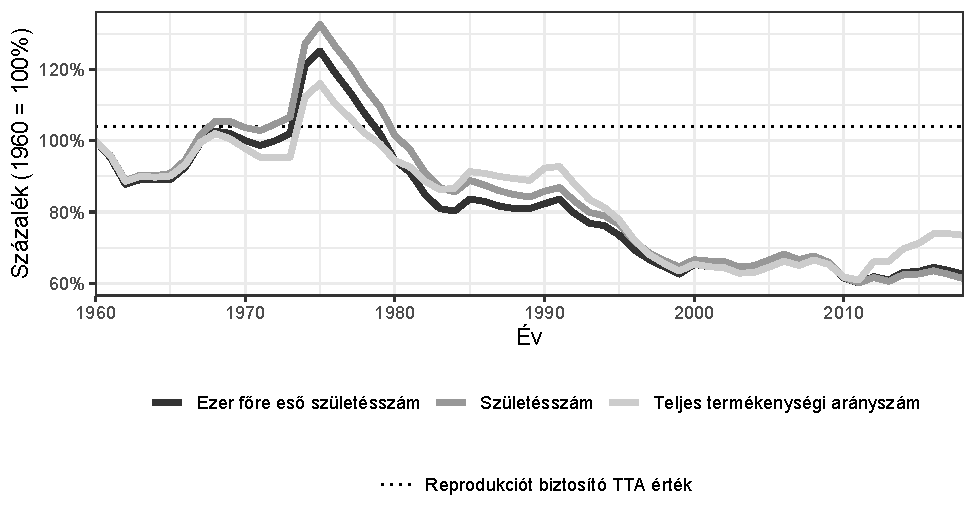
\includegraphics{ujdemografiaiprogram_files/figure-latex/unnamed-chunk-2-1.pdf}
\caption{Magyar születési mutatók bázisindexe (1960 = 100\%)}
\end{figure}

\begin{figure}
\centering
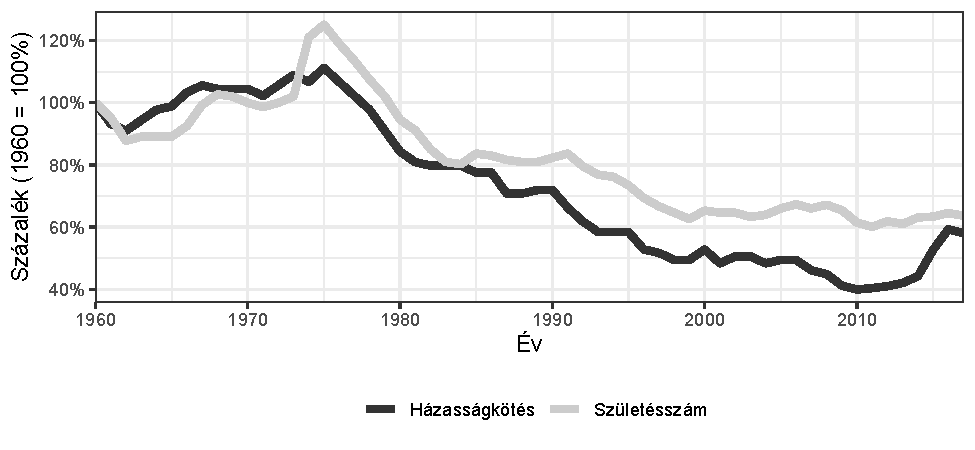
\includegraphics{ujdemografiaiprogram_files/figure-latex/unnamed-chunk-3-1.pdf}
\caption{A születésszám és házasság kötések ezer főre eső számának
bázisindexe}
\end{figure}

\begin{figure}
\centering
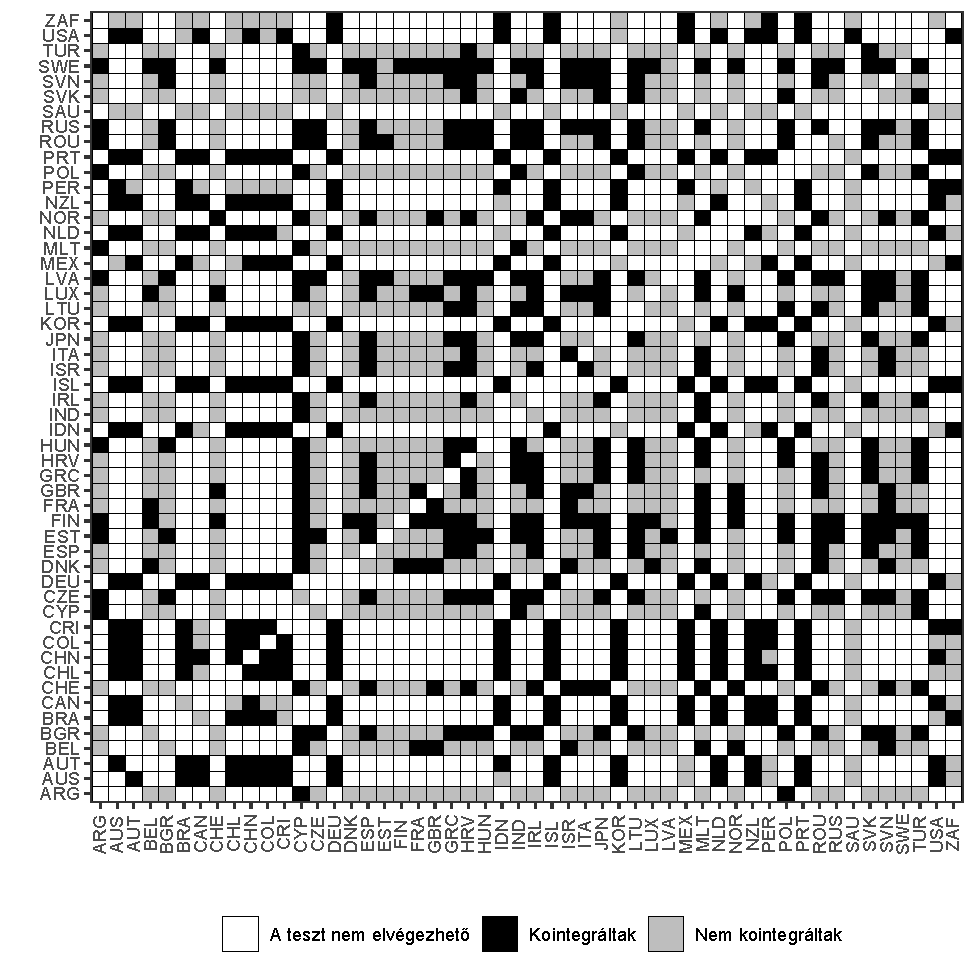
\includegraphics{ujdemografiaiprogram_files/figure-latex/unnamed-chunk-8-1.pdf}
\caption{Kointegrációs tesztek eredményei}
\end{figure}

\begin{longtable}[]{@{}lcc@{}}
\caption{Tesztek eredményeinek arányai egymással határos és nem határos
országok esetében}\tabularnewline
\toprule
& Határosak & Nem határosak\tabularnewline
\midrule
\endfirsthead
\toprule
& Határosak & Nem határosak\tabularnewline
\midrule
\endhead
A teszt nem elvégezhető & 32,9\% & 49,3\%\tabularnewline
Nem kointegráltak & 28,2\% & 27,9\%\tabularnewline
Kointegráltak & 38,8\% & 22,8\%\tabularnewline
\bottomrule
\end{longtable}

\begin{figure}
\centering
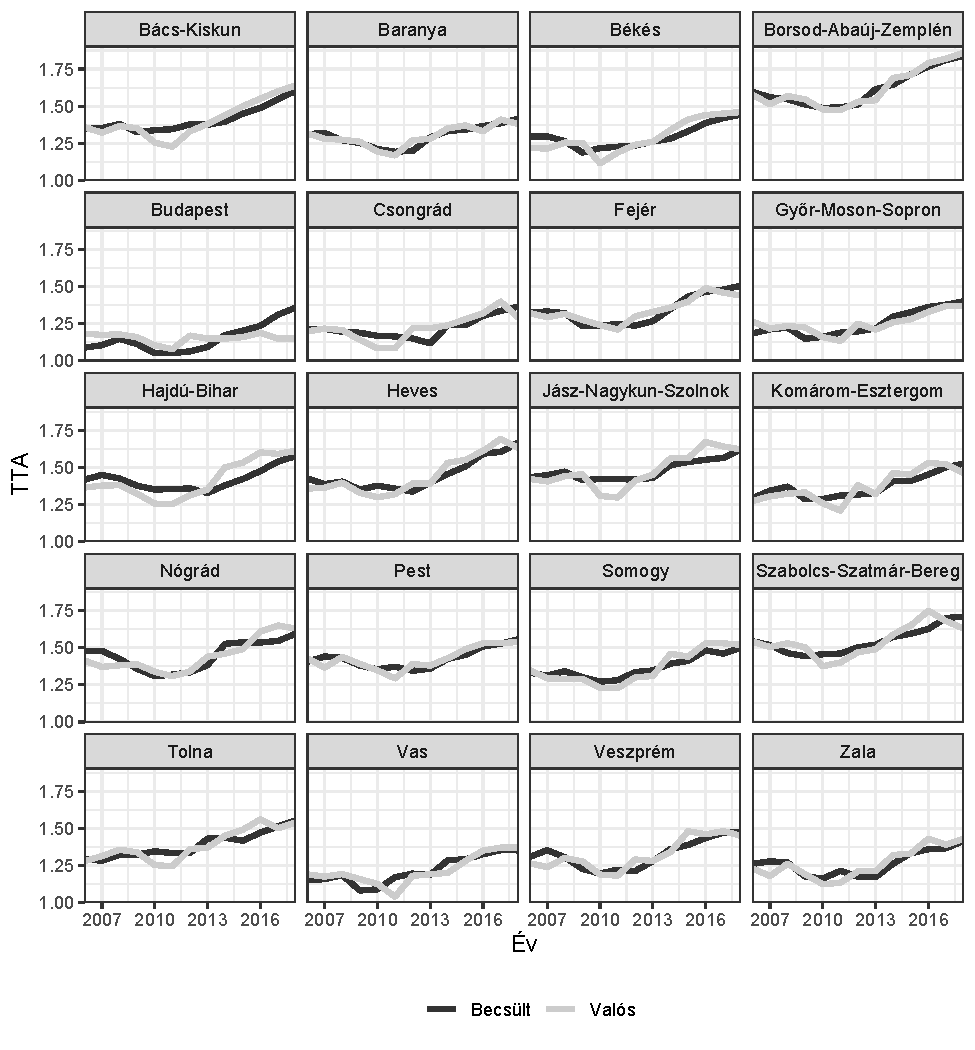
\includegraphics{ujdemografiaiprogram_files/figure-latex/unnamed-chunk-14-1.pdf}
\caption{TTA becslése megyénként a fix modellel}
\end{figure}

\begin{figure}
\centering
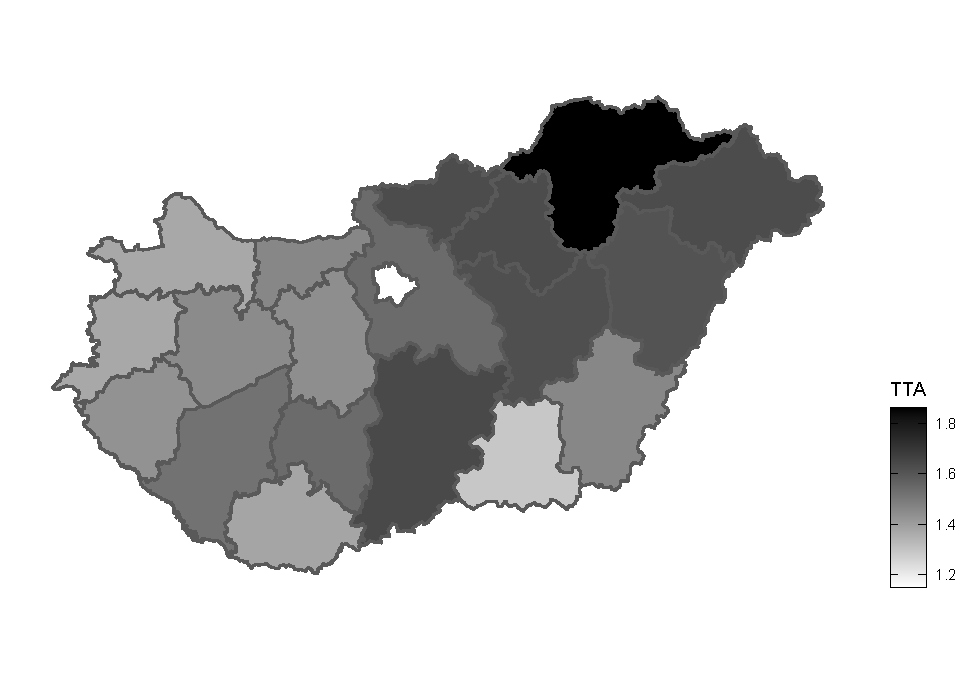
\includegraphics{ujdemografiaiprogram_files/figure-latex/unnamed-chunk-15-1.pdf}
\caption{A teljes termékenységi arányszám 2018-ban megyénként}
\end{figure}

\begin{landscape}\begin{table}

\caption{\label{tab:unnamed-chunk-18}Panel}
\centering
\begin{tabular}[t]{l|l|c|c|c|c}
\hline
\multicolumn{1}{c|}{ } & \multicolumn{2}{c|}{I} & \multicolumn{2}{c}{II} \\
\cline{2-3} \cline{4-5}
 &  & változó & p-érték & változó & p-érték\\
\hline
 & GDP/fő & 0.000195805817665817 & 0.00\% & 6.33562999839744e-05 & 0.00\%\\
\cline{2-6}
 & GDP/fő\textasciicircum{}2 & -1.60664424208637e-08 & 0.00\% &  & \\
\cline{2-6}
 & GDP/fő (l=1) &  &  &  & \\
\cline{2-6}
 & GDP/fő (l=1)\textasciicircum{}2 &  &  &  & \\
\cline{2-6}
 & Munkanélküliségi ráta & -0.0159192191149856 & 0.00\% & -0.0205144668884857 & 0.00\%\\
\cline{2-6}
 & Munkanélküliségi ráta\textasciicircum{}2 &  &  &  & \\
\cline{2-6}
 & Munkanélküliségi ráta (l=1) &  &  &  & \\
\cline{2-6}
\multirow[t]{-8}{*}{\raggedright\arraybackslash a} & Munkanélküliségi ráta (l=1)\textasciicircum{}2 &  &  &  & \\
\cline{1-6}
 & Chow-teszt &  & 0.00\% &  & 0.00\%\\
\cline{2-6}
 & Hausman-teszt &  & 0.00\% &  & 0.00\%\\
\cline{2-6}
\multirow[t]{-3}{*}{\raggedright\arraybackslash b} & Korrigált R\textasciicircum{}2 &  & 76.04\% &  & 68.07\%\\
\hline
\end{tabular}
\end{table}
\end{landscape}

\begin{figure}
\centering
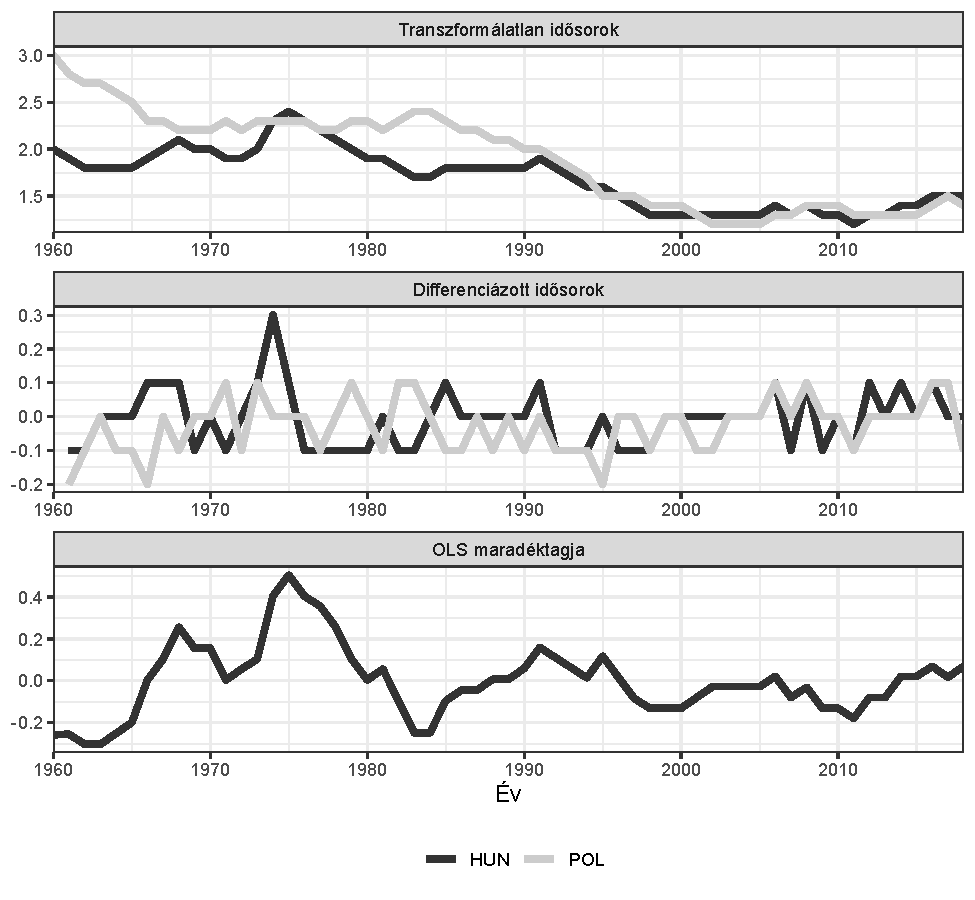
\includegraphics{ujdemografiaiprogram_files/figure-latex/unnamed-chunk-19-1.pdf}
\caption{A magyar és lengyel TTA idősorok között fennálló kointegráció}
\end{figure}

\pagebreak

\nocite{*}

\bibliography{ujdemografiaiprogram}
\bibliographystyle{agsm}

\hypertarget{fuxfcggeluxe9k}{%
\section{Függelék}\label{fuxfcggeluxe9k}}

\hypertarget{a-tanulmuxe1ny-elkuxe9szuxedtuxe9suxe9hez-hasznuxe1lt-r-kuxf3dok}{%
\subsection{A tanulmány elkészítéséhez használt R
kódok}\label{a-tanulmuxe1ny-elkuxe9szuxedtuxe9suxe9hez-hasznuxe1lt-r-kuxf3dok}}

\begin{Shaded}
\begin{Highlighting}[numbers=left,,]
\CommentTok{# packages and setup --------------------------------------------------------------------}
\KeywordTok{library}\NormalTok{(ggpubr)}
\KeywordTok{library}\NormalTok{(tseries)}
\KeywordTok{library}\NormalTok{(forecast)}
\KeywordTok{library}\NormalTok{(plm)}
\KeywordTok{library}\NormalTok{(sf)}
\KeywordTok{library}\NormalTok{(tidyverse)}
\KeywordTok{theme_set}\NormalTok{(}\KeywordTok{theme_bw}\NormalTok{() }\OperatorTok{+}\StringTok{ }\KeywordTok{theme}\NormalTok{(}\DataTypeTok{legend.position =} \StringTok{"bottom"}\NormalTok{))}
\KeywordTok{load}\NormalTok{(}\StringTok{"ujdemografiaiprogram.RData"}\NormalTok{)}
\KeywordTok{options}\NormalTok{(}\DataTypeTok{knitr.kable.NA =} \StringTok{''}\NormalTok{) }
\CommentTok{# Figure 1 ------------------------------------------------------------------------------}
\NormalTok{LiveBirthAndFertility }\OperatorTok\StringTok{ }
\StringTok{  }\KeywordTok{mutate_at}\NormalTok{(}\OperatorTok{-}\DecValTok{1}\NormalTok{, }\ControlFlowTok{function}\NormalTok{(x) x}\OperatorTok{/}\NormalTok{x[}\DecValTok{1}\NormalTok{]) }\OperatorTok\StringTok{ }
\StringTok{  }\KeywordTok{pivot_longer}\NormalTok{(}\OperatorTok{-}\DecValTok{1}\NormalTok{) }\OperatorTok\StringTok{ }\KeywordTok{mutate}\NormalTok{(}
    \DataTypeTok{name =} \KeywordTok{case_when}\NormalTok{(}
\NormalTok{      name }\OperatorTok{==}\StringTok{ "LiveBirthTotal"} \OperatorTok{~}\StringTok{ "Születésszám"}\NormalTok{,}
\NormalTok{      name }\OperatorTok{==}\StringTok{ "LiveBirthTo1000"} \OperatorTok{~}\StringTok{ "Ezer főre eső születésszám"}\NormalTok{,}
\NormalTok{      T }\OperatorTok{~}\StringTok{ "Teljes termékenységi arányszám"}
\NormalTok{    )}
\NormalTok{  ) }\OperatorTok\StringTok{ }\KeywordTok{ggplot}\NormalTok{() }\OperatorTok{+}\StringTok{ }
\StringTok{  }\KeywordTok{geom_hline}\NormalTok{(}\KeywordTok{aes}\NormalTok{(}\DataTypeTok{yintercept =} \FloatTok{2.1}\OperatorTok{/}\NormalTok{LiveBirthAndFertility}\OperatorTok{$}\NormalTok{TotalFertility[}\DecValTok{1}\NormalTok{],}
                 \DataTypeTok{linetype =} \StringTok{"Reprodukciót biztosító TTA érték"}\NormalTok{), }\DataTypeTok{color =} \StringTok{"black"}\NormalTok{) }\OperatorTok{+}\StringTok{ }
\StringTok{  }\KeywordTok{geom_line}\NormalTok{(}\KeywordTok{aes}\NormalTok{(}\DataTypeTok{x =}\NormalTok{ Year, }\DataTypeTok{y =}\NormalTok{ value, }\DataTypeTok{color =}\NormalTok{ name), }\DataTypeTok{size =} \FloatTok{1.3}\NormalTok{) }\OperatorTok{+}\StringTok{ }
\StringTok{  }\KeywordTok{scale_color_grey}\NormalTok{() }\OperatorTok{+}\StringTok{ }
\StringTok{  }\KeywordTok{scale_linetype_manual}\NormalTok{(}\DataTypeTok{values =} \KeywordTok{c}\NormalTok{(}\StringTok{"Reprodukciót biztosító TTA érték"}\NormalTok{ =}\StringTok{ "dotted"}\NormalTok{)) }\OperatorTok{+}
\StringTok{  }\KeywordTok{scale_x_continuous}\NormalTok{(}\DataTypeTok{expand =} \KeywordTok{c}\NormalTok{(}\DecValTok{0}\NormalTok{,}\DecValTok{0}\NormalTok{)) }\OperatorTok{+}\StringTok{ }
\StringTok{  }\KeywordTok{scale_y_continuous}\NormalTok{(}\DataTypeTok{labels =}\NormalTok{ scales}\OperatorTok{::}\NormalTok{percent) }\OperatorTok{+}\StringTok{ }
\StringTok{  }\KeywordTok{labs}\NormalTok{(}\DataTypeTok{x =} \StringTok{"Év"}\NormalTok{, }\DataTypeTok{y =} \StringTok{"Százalék (1960 = 100%)"}\NormalTok{, }\DataTypeTok{color =} \OtherTok{NULL}\NormalTok{, }\DataTypeTok{linetype =} \OtherTok{NULL}\NormalTok{) }\OperatorTok{+}
\StringTok{  }\KeywordTok{theme}\NormalTok{(}\DataTypeTok{legend.box =} \StringTok{"vertical"}\NormalTok{)}

\CommentTok{# Figure 2 ------------------------------------------------------------------------------}
\KeywordTok{merge}\NormalTok{(socioeconomic_indicators[,}\KeywordTok{c}\NormalTok{(}\StringTok{"Year"}\NormalTok{, }\StringTok{"Marriage"}\NormalTok{)],}
\NormalTok{      LiveBirthAndFertility[,}\KeywordTok{c}\NormalTok{(}\StringTok{"Year"}\NormalTok{,}\StringTok{"LiveBirthTo1000"}\NormalTok{)]}
\NormalTok{) }\OperatorTok
\StringTok{  }\KeywordTok{mutate_at}\NormalTok{(}\OperatorTok{-}\DecValTok{1}\NormalTok{, }\ControlFlowTok{function}\NormalTok{(x) x}\OperatorTok{/}\NormalTok{x[}\DecValTok{1}\NormalTok{]) }\OperatorTok\StringTok{ }\KeywordTok{pivot_longer}\NormalTok{(}\OperatorTok{-}\DecValTok{1}\NormalTok{) }\OperatorTok\StringTok{ }
\StringTok{  }\KeywordTok{mutate}\NormalTok{(}\DataTypeTok{name =} \KeywordTok{ifelse}\NormalTok{(name }\OperatorTok{==}\StringTok{ "Marriage"}\NormalTok{, }\StringTok{"Házasságkötés"}\NormalTok{, }\StringTok{"Születésszám"}\NormalTok{)) }\OperatorTok\StringTok{ }
\StringTok{  }\KeywordTok{ggplot}\NormalTok{() }\OperatorTok{+}\StringTok{  }\KeywordTok{geom_line}\NormalTok{(}\KeywordTok{aes}\NormalTok{(}\DataTypeTok{x =}\NormalTok{ Year, }\DataTypeTok{y =}\NormalTok{ value, }\DataTypeTok{color =}\NormalTok{ name), }\DataTypeTok{size =} \FloatTok{1.7}\NormalTok{) }\OperatorTok{+}\StringTok{ }
\StringTok{  }\KeywordTok{scale_color_grey}\NormalTok{() }\OperatorTok{+}\StringTok{ }\KeywordTok{scale_x_continuous}\NormalTok{(}\DataTypeTok{expand =} \KeywordTok{c}\NormalTok{(}\DecValTok{0}\NormalTok{,}\DecValTok{0}\NormalTok{)) }\OperatorTok{+}\StringTok{ }
\StringTok{  }\KeywordTok{scale_y_continuous}\NormalTok{(}\DataTypeTok{labels =}\NormalTok{ scales}\OperatorTok{::}\NormalTok{percent) }\OperatorTok{+}\StringTok{ }
\StringTok{  }\KeywordTok{labs}\NormalTok{(}\DataTypeTok{x =} \StringTok{"Év"}\NormalTok{, }\DataTypeTok{y =} \StringTok{"Százalék (1960 = 100%)"}\NormalTok{, }\DataTypeTok{color =} \OtherTok{NULL}\NormalTok{)}

\CommentTok{# OECD data import ----------------------------------------------------------------------}
\NormalTok{oecd_fertility <-}\StringTok{ }\CommentTok{# Total Fertility Rate (children/woman) from OECD webpage}
\StringTok{  }\KeywordTok{read.csv}\NormalTok{(}\KeywordTok{paste0}\NormalTok{(}
    \StringTok{"https://stats.oecd.org/sdmx-json/data/DP_LIVE/.FERTILITY.TOT.CHD_WOMAN.A/OECD?"}\NormalTok{,}
    \StringTok{"contentType=csv&detail=code&separator=comma&csv-lang=en&startPeriod="}\NormalTok{,}
    \StringTok{"1960&endPeriod=2019"}\NormalTok{)) }\OperatorTok
\StringTok{  }\NormalTok{dplyr}\OperatorTok{::}\KeywordTok{select}\NormalTok{(}\DecValTok{1}\NormalTok{,}\DecValTok{6}\NormalTok{,}\DecValTok{7}\NormalTok{) }\OperatorTok\StringTok{ }\KeywordTok{set_names}\NormalTok{(}\KeywordTok{c}\NormalTok{(}\StringTok{"location"}\NormalTok{, }\StringTok{"time"}\NormalTok{, }\StringTok{"tfr"}\NormalTok{))}

\NormalTok{oecd_GDPcap <-}\StringTok{ }\CommentTok{# GDP/cap (dollar) from OECD webpage}
\StringTok{  }\KeywordTok{read.csv}\NormalTok{(}\KeywordTok{paste0}\NormalTok{(}
    \StringTok{"https://stats.oecd.org/sdmx-json/data/DP_LIVE/.GDP.TOT.USD_CAP.A/OECD?contentType"}\NormalTok{,}
    \StringTok{"=csv&detail=code&separator=comma&csv-lang=en&startPeriod=1960&endPeriod=2019"}\NormalTok{)) }\OperatorTok
\StringTok{  }\NormalTok{dplyr}\OperatorTok{::}\KeywordTok{select}\NormalTok{(}\DecValTok{1}\NormalTok{,}\DecValTok{6}\NormalTok{,}\DecValTok{7}\NormalTok{) }\OperatorTok\StringTok{ }\KeywordTok{set_names}\NormalTok{(}\KeywordTok{c}\NormalTok{(}\StringTok{"location"}\NormalTok{, }\StringTok{"time"}\NormalTok{, }\StringTok{"GDPcap"}\NormalTok{))}

\CommentTok{# Figure x ------------------------------------------------------------------------------}
\NormalTok{v <-}\StringTok{ }\KeywordTok{vector}\NormalTok{()}
\ControlFlowTok{for}\NormalTok{ (i }\ControlFlowTok{in} \DecValTok{1960}\OperatorTok{:}\DecValTok{2019}\NormalTok{) \{}
\NormalTok{  v[i }\OperatorTok{-}\StringTok{ }\DecValTok{1959}\NormalTok{] <-}\StringTok{ }\KeywordTok{merge}\NormalTok{(oecd_fertility,oecd_GDPcap) }\OperatorTok
\StringTok{    }\KeywordTok{filter}\NormalTok{(time }\OperatorTok{==}\StringTok{ }\NormalTok{i }\OperatorTok{&}\StringTok{ }\NormalTok{location }\OperatorTok{!=}\StringTok{ "OAVG"} \OperatorTok{&}\StringTok{ }\NormalTok{location }\OperatorTok{!=}\StringTok{ "EU"}\NormalTok{) }\OperatorTok
\StringTok{    }\NormalTok{dplyr}\OperatorTok{::}\KeywordTok{select}\NormalTok{(tfr, GDPcap) }\OperatorTok\StringTok{ }\KeywordTok{cor}\NormalTok{() }\OperatorTok\StringTok{ }\NormalTok{.[}\DecValTok{1}\NormalTok{,}\DecValTok{2}\NormalTok{]}
\NormalTok{\}}

\KeywordTok{ggplot}\NormalTok{(}\DataTypeTok{data =} \KeywordTok{data.frame}\NormalTok{(}\DataTypeTok{time =} \DecValTok{1960}\OperatorTok{:}\DecValTok{2019}\NormalTok{, }\DataTypeTok{y =}\NormalTok{ v)) }\OperatorTok{+}
\StringTok{  }\KeywordTok{geom_hline}\NormalTok{(}\DataTypeTok{yintercept =} \DecValTok{0}\NormalTok{) }\OperatorTok{+}\StringTok{ }
\StringTok{  }\KeywordTok{geom_col}\NormalTok{(}\KeywordTok{aes}\NormalTok{(}\DataTypeTok{x =}\NormalTok{ time, }\DataTypeTok{y =}\NormalTok{ y), }\DataTypeTok{fill =} \StringTok{"grey70"}\NormalTok{, }\DataTypeTok{color =} \StringTok{"black"}\NormalTok{) }\OperatorTok{+}
\StringTok{  }\KeywordTok{geom_line}\NormalTok{(}\KeywordTok{aes}\NormalTok{(}\DataTypeTok{x =}\NormalTok{ time, }\DataTypeTok{y =} 
                  \KeywordTok{merge}\NormalTok{(oecd_fertility,oecd_GDPcap) }\OperatorTok
\StringTok{                  }\KeywordTok{filter}\NormalTok{(location }\OperatorTok{!=}\StringTok{ "OAVG"} \OperatorTok{&}\StringTok{ }\NormalTok{location }\OperatorTok{!=}\StringTok{ "EU"}\NormalTok{) }\OperatorTok
\StringTok{                  }\KeywordTok{group_by}\NormalTok{(time) }\OperatorTok\StringTok{ }\KeywordTok{summarize}\NormalTok{(}\DataTypeTok{n =} \KeywordTok{n}\NormalTok{()) }\OperatorTok\StringTok{ }\KeywordTok{mutate}\NormalTok{(}\DataTypeTok{n =}\NormalTok{ n}\OperatorTok{/}\KeywordTok{max}\NormalTok{(n)) }\OperatorTok
\StringTok{                  }\NormalTok{.}\OperatorTok{$}\NormalTok{n, }\DataTypeTok{color =} \StringTok{"Adatok aránya (52 országról elérhető adat = 1)"}\NormalTok{)) }\OperatorTok{+}\StringTok{ }
\StringTok{  }\CommentTok{#labs(y = "Lineáris korrelációs együttható", x = "Év", color = NULL) +}
\StringTok{  }\KeywordTok{scale_y_continuous}\NormalTok{(}\DataTypeTok{limits =} \KeywordTok{c}\NormalTok{(}\OperatorTok{-}\DecValTok{1}\NormalTok{,}\DecValTok{1}\NormalTok{), }\DataTypeTok{expand =} \KeywordTok{c}\NormalTok{(}\DecValTok{0}\NormalTok{,}\DecValTok{0}\NormalTok{)) }\OperatorTok{+}
\StringTok{  }\KeywordTok{scale_color_grey}\NormalTok{()}

\CommentTok{# Neighbourhood effect ----------------------------------------------------------------}
\NormalTok{df <-}\StringTok{ }\NormalTok{NeighbourCountry }\OperatorTok\StringTok{ }\KeywordTok{mutate}\NormalTok{(}\DataTypeTok{x =} \KeywordTok{names}\NormalTok{(NeighbourCountry)) }\OperatorTok
\StringTok{  }\KeywordTok{pivot_longer}\NormalTok{(}\OperatorTok{-}\NormalTok{x, }\DataTypeTok{names_to =} \StringTok{"y"}\NormalTok{, }\DataTypeTok{values_to =} \StringTok{"neighbour"}\NormalTok{) }\OperatorTok\StringTok{ }\KeywordTok{mutate}\NormalTok{(}
    \DataTypeTok{neighbour =} \KeywordTok{ifelse}\NormalTok{(}\KeywordTok{is.na}\NormalTok{(neighbour), }\StringTok{"Nem határosak"}\NormalTok{, }\StringTok{"Határosak"}\NormalTok{),}
    \DataTypeTok{neighbour =} \KeywordTok{ifelse}\NormalTok{(x }\OperatorTok{==}\StringTok{ }\NormalTok{y, }\OtherTok{NA}\NormalTok{, neighbour)}
\NormalTok{  ) }\OperatorTok\StringTok{ }\KeywordTok{merge}\NormalTok{(}
\NormalTok{    oecd_fertility }\OperatorTok\StringTok{ }\KeywordTok{group_by}\NormalTok{(location) }\OperatorTok
\StringTok{      }\KeywordTok{summarise}\NormalTok{(}\DataTypeTok{d =} \KeywordTok{ndiffs}\NormalTok{(tfr, }\DataTypeTok{test =} \StringTok{"kpss"}\NormalTok{, }\DataTypeTok{type =} \StringTok{"level"}\NormalTok{, }\DataTypeTok{alpha =} \FloatTok{.05}\NormalTok{)) }\OperatorTok
\StringTok{      }\KeywordTok{set_names}\NormalTok{(}\StringTok{"y"}\NormalTok{, }\StringTok{"dy"}\NormalTok{)}
\NormalTok{  ) }\OperatorTok\StringTok{ }\KeywordTok{merge}\NormalTok{(}
\NormalTok{    oecd_fertility }\OperatorTok\StringTok{ }\KeywordTok{group_by}\NormalTok{(location) }\OperatorTok
\StringTok{      }\KeywordTok{summarise}\NormalTok{(}\DataTypeTok{d =} \KeywordTok{ndiffs}\NormalTok{(tfr, }\DataTypeTok{test =} \StringTok{"kpss"}\NormalTok{, }\DataTypeTok{type =} \StringTok{"level"}\NormalTok{, }\DataTypeTok{alpha =} \FloatTok{.05}\NormalTok{)) }\OperatorTok
\StringTok{      }\KeywordTok{set_names}\NormalTok{(}\StringTok{"x"}\NormalTok{, }\StringTok{"dx"}\NormalTok{)}
\NormalTok{  )}

\NormalTok{v <-}\StringTok{ }\KeywordTok{vector}\NormalTok{() }\CommentTok{# collector vector}
\ControlFlowTok{for}\NormalTok{ (i }\ControlFlowTok{in} \DecValTok{1}\OperatorTok{:}\KeywordTok{nrow}\NormalTok{(df)) \{}
  \ControlFlowTok{if}\NormalTok{ (df}\OperatorTok{$}\NormalTok{dx[i] }\OperatorTok{==}\StringTok{ }\NormalTok{df}\OperatorTok{$}\NormalTok{dy[i] }\OperatorTok{&}\StringTok{ }\NormalTok{df}\OperatorTok{$}\NormalTok{x[i] }\OperatorTok{!=}\StringTok{ }\NormalTok{df}\OperatorTok{$}\NormalTok{y[i]) \{}
\NormalTok{    res <-}\StringTok{ }\NormalTok{oecd_fertility }\OperatorTok
\StringTok{      }\KeywordTok{pivot_wider}\NormalTok{(}\DataTypeTok{names_from =} \StringTok{"location"}\NormalTok{, }\DataTypeTok{values_from =} \StringTok{"tfr"}\NormalTok{) }\OperatorTok
\StringTok{      }\NormalTok{dplyr}\OperatorTok{::}\KeywordTok{select}\NormalTok{(df}\OperatorTok{$}\NormalTok{x[i],  df}\OperatorTok{$}\NormalTok{y[i]) }\OperatorTok\StringTok{ }\KeywordTok{set_names}\NormalTok{(}\KeywordTok{c}\NormalTok{(}\StringTok{"x"}\NormalTok{, }\StringTok{"y"}\NormalTok{)) }\OperatorTok
\StringTok{      }\KeywordTok{na.exclude}\NormalTok{() }\OperatorTok\StringTok{ }\KeywordTok{lm}\NormalTok{(}\DataTypeTok{formula =}\NormalTok{ y }\OperatorTok{~}\StringTok{ }\NormalTok{x) }\OperatorTok\StringTok{ }\NormalTok{.}\OperatorTok{$}\NormalTok{residuals}
    
    \ControlFlowTok{if}\NormalTok{ (}\KeywordTok{ndiffs}\NormalTok{(res , }\DataTypeTok{test =} \StringTok{"kpss"}\NormalTok{, }\DataTypeTok{type =} \StringTok{"level"}\NormalTok{, }\DataTypeTok{alpha =} \FloatTok{.05}\NormalTok{) }\OperatorTok{<}\StringTok{ }\NormalTok{df}\OperatorTok{$}\NormalTok{dx[i]) \{}
\NormalTok{      v[i] <-}\StringTok{  "Kointegráltak"}  
\NormalTok{    \} }\ControlFlowTok{else}\NormalTok{ \{}
\NormalTok{      v[i] <-}\StringTok{  "Nem kointegráltak"}
\NormalTok{    \}}
\NormalTok{  \} }\ControlFlowTok{else}\NormalTok{ \{}
\NormalTok{    v[i] <-}\StringTok{  "A teszt nem elvégezhető"}  
\NormalTok{  \}}
\NormalTok{\}}

\NormalTok{df}\OperatorTok{$}\NormalTok{coint <-}\StringTok{ }\NormalTok{v}

\NormalTok{df <-}\StringTok{ }\KeywordTok{merge}\NormalTok{(df, oecd_fertility }\OperatorTok
\StringTok{              }\KeywordTok{pivot_wider}\NormalTok{(}\DataTypeTok{names_from =} \StringTok{"location"}\NormalTok{, }\DataTypeTok{values_from =} \StringTok{"tfr"}\NormalTok{) }\OperatorTok
\StringTok{              }\NormalTok{dplyr}\OperatorTok{::}\KeywordTok{select}\NormalTok{(}\OperatorTok{-}\DecValTok{1}\NormalTok{) }\OperatorTok\StringTok{ }\KeywordTok{cor}\NormalTok{(}\DataTypeTok{use =} \StringTok{"pairwise.complete.obs"}\NormalTok{) }\OperatorTok
\StringTok{              }\KeywordTok{data.frame}\NormalTok{() }\OperatorTok\StringTok{ }\KeywordTok{rownames_to_column}\NormalTok{(}\DataTypeTok{var =} \StringTok{"x"}\NormalTok{) }\OperatorTok\StringTok{ }
\StringTok{              }\KeywordTok{pivot_longer}\NormalTok{(}\OperatorTok{-}\DecValTok{1}\NormalTok{, }\DataTypeTok{names_to =} \StringTok{"y"}\NormalTok{, }\DataTypeTok{values_to =} \StringTok{"cor"}\NormalTok{))}

\NormalTok{df }\OperatorTok\StringTok{ }\KeywordTok{group_by}\NormalTok{(neighbour) }\OperatorTok\StringTok{ }\KeywordTok{summarise}\NormalTok{(}\KeywordTok{mean}\NormalTok{(cor)) }\CommentTok{# mean of correlation}

\CommentTok{# Figure 3 ------------------------------------------------------------------------------}
\KeywordTok{ggplot}\NormalTok{(}\DataTypeTok{data =}\NormalTok{ df) }\OperatorTok{+}\StringTok{ }\KeywordTok{geom_tile}\NormalTok{(}\KeywordTok{aes}\NormalTok{(}\DataTypeTok{x =}\NormalTok{ x, }\DataTypeTok{y =}\NormalTok{ y, }\DataTypeTok{fill =}\NormalTok{ coint), }\DataTypeTok{color =} \StringTok{"black"}\NormalTok{) }\OperatorTok{+}\StringTok{ }
\StringTok{  }\KeywordTok{labs}\NormalTok{(}\DataTypeTok{x =} \StringTok{""}\NormalTok{, }\DataTypeTok{y =} \StringTok{""}\NormalTok{, }\DataTypeTok{fill =} \StringTok{""}\NormalTok{) }\OperatorTok{+}
\StringTok{  }\KeywordTok{scale_fill_manual}\NormalTok{(}\DataTypeTok{values =} \KeywordTok{c}\NormalTok{(}\StringTok{"white"}\NormalTok{, }\StringTok{"black"}\NormalTok{, }\StringTok{"grey"}\NormalTok{)) }\OperatorTok{+}
\StringTok{  }\KeywordTok{theme}\NormalTok{(}\DataTypeTok{axis.text.x =} \KeywordTok{element_text}\NormalTok{(}\DataTypeTok{angle =} \DecValTok{90}\NormalTok{, }\DataTypeTok{vjust =} \FloatTok{0.45}\NormalTok{))}

\NormalTok{df }\OperatorTok\StringTok{ }\KeywordTok{group_by}\NormalTok{(neighbour, coint) }\OperatorTok\StringTok{ }\KeywordTok{summarise}\NormalTok{(}\DataTypeTok{n =} \KeywordTok{n}\NormalTok{()) }\OperatorTok\StringTok{ }\KeywordTok{filter}\NormalTok{(}\OperatorTok{!}\KeywordTok{is.na}\NormalTok{(neighbour)) }\OperatorTok\StringTok{ }
\StringTok{  }\KeywordTok{pivot_wider}\NormalTok{(}\DataTypeTok{names_from =}\NormalTok{ neighbour, }\DataTypeTok{values_from =}\NormalTok{ n) }\OperatorTok
\StringTok{  }\KeywordTok{mutate_at}\NormalTok{(}\OperatorTok{-}\DecValTok{1}\NormalTok{, }\ControlFlowTok{function}\NormalTok{(x) scales}\OperatorTok{::}\KeywordTok{percent}\NormalTok{(x}\OperatorTok{/}\KeywordTok{sum}\NormalTok{(x), }\DataTypeTok{decimal.mark =} \StringTok{","}\NormalTok{)) }\OperatorTok
\StringTok{  }\NormalTok{.[}\KeywordTok{c}\NormalTok{(}\DecValTok{1}\NormalTok{,}\DecValTok{3}\NormalTok{,}\DecValTok{2}\NormalTok{),] }\OperatorTok\StringTok{ }
\StringTok{  }\NormalTok{knitr}\OperatorTok{::}\KeywordTok{kable}\NormalTok{(}\DataTypeTok{col.names =} \KeywordTok{c}\NormalTok{(}\StringTok{""}\NormalTok{, }\StringTok{"Határosak"}\NormalTok{, }\StringTok{"Nem határosak"}\NormalTok{), }\DataTypeTok{align =} \KeywordTok{c}\NormalTok{(}\StringTok{"l"}\NormalTok{, }\StringTok{"c"}\NormalTok{, }\StringTok{"c"}\NormalTok{),}
    \DataTypeTok{caption =} 
    \StringTok{"Tesztek eredményeinek arányai egymással határos és nem határos országok esetében"}\NormalTok{)}

\KeywordTok{merge}\NormalTok{(oecd_fertility,oecd_GDPcap) }\OperatorTok\StringTok{ }\KeywordTok{ggplot}\NormalTok{(}\KeywordTok{aes}\NormalTok{(}\DataTypeTok{x =}\NormalTok{ GDPcap, }\DataTypeTok{y =}\NormalTok{ tfr)) }\OperatorTok{+}
\StringTok{  }\KeywordTok{geom_point}\NormalTok{(}\DataTypeTok{shape =} \DecValTok{21}\NormalTok{, }\DataTypeTok{alpha =} \FloatTok{.8}\NormalTok{, }\DataTypeTok{fill =} \StringTok{"grey70"}\NormalTok{) }\OperatorTok{+}
\StringTok{  }\KeywordTok{geom_smooth}\NormalTok{(}\DataTypeTok{se =}\NormalTok{ F, }\DataTypeTok{size =} \FloatTok{1.7}\NormalTok{, }\DataTypeTok{color =} \StringTok{"black"}\NormalTok{, }\DataTypeTok{formula =}\NormalTok{ y }\OperatorTok{~}\StringTok{ }\NormalTok{x }\OperatorTok{+}\StringTok{ }\NormalTok{x}\OperatorTok{^}\DecValTok{2}\NormalTok{) }\OperatorTok{+}\StringTok{ }
\StringTok{  }\NormalTok{gganimate}\OperatorTok{::}\KeywordTok{transition_time}\NormalTok{(time) }\OperatorTok{+}\StringTok{ }\KeywordTok{labs}\NormalTok{(}\DataTypeTok{title =} \StringTok{'\{frame_time\}'}\NormalTok{)}

\CommentTok{# Chow and Hausman-test -----------------------------------------------------------------}
\NormalTok{c.panel.pooling <-}\StringTok{ }\KeywordTok{plm}\NormalTok{(}\DataTypeTok{formula =}\NormalTok{ tfr }\OperatorTok{~}\StringTok{ }\NormalTok{GDPcap }\OperatorTok{+}\StringTok{ }\NormalTok{unr, }\DataTypeTok{data =}\NormalTok{ c.panel, }\DataTypeTok{model =} \StringTok{"pooling"}\NormalTok{)}
\NormalTok{c.panel.within <-}\StringTok{ }\KeywordTok{plm}\NormalTok{(}\DataTypeTok{formula =}\NormalTok{ tfr }\OperatorTok{~}\StringTok{ }\NormalTok{GDPcap }\OperatorTok{+}\StringTok{ }\NormalTok{unr, }\DataTypeTok{data =}\NormalTok{ c.panel, }\DataTypeTok{model =} \StringTok{"within"}\NormalTok{)}
\NormalTok{c.panel.random <-}\StringTok{ }\KeywordTok{plm}\NormalTok{(}\DataTypeTok{formula =}\NormalTok{ tfr }\OperatorTok{~}\StringTok{ }\NormalTok{GDPcap }\OperatorTok{+}\StringTok{ }\NormalTok{unr, }\DataTypeTok{data =}\NormalTok{ c.panel, }\DataTypeTok{model =} \StringTok{"random"}\NormalTok{)}
\KeywordTok{pooltest}\NormalTok{(c.panel.pooling, c.panel.within)}
\KeywordTok{phtest}\NormalTok{(c.panel.within, c.panel.random)}

\CommentTok{# Hungarian map draw function -----------------------------------------------------------}
\NormalTok{hun_map_plot <-}\StringTok{ }\ControlFlowTok{function}\NormalTok{(df, }\DataTypeTok{na.value =} \StringTok{"white"}\NormalTok{, }\DataTypeTok{low =} \StringTok{"white"}\NormalTok{, }\DataTypeTok{high =} \StringTok{"black"}\NormalTok{) \{}
\NormalTok{  hunsf }\OperatorTok\StringTok{ }\KeywordTok{merge}\NormalTok{(}\KeywordTok{set_names}\NormalTok{(df, }\KeywordTok{c}\NormalTok{(}\StringTok{"NAME"}\NormalTok{, }\StringTok{"value"}\NormalTok{))) }\OperatorTok\StringTok{  }\KeywordTok{ggplot}\NormalTok{() }\OperatorTok{+}
\StringTok{    }\KeywordTok{geom_sf}\NormalTok{(}\KeywordTok{aes}\NormalTok{(}\DataTypeTok{fill =}\NormalTok{ value)) }\OperatorTok{+}\StringTok{ }\NormalTok{ggthemes}\OperatorTok{::}\KeywordTok{theme_map}\NormalTok{() }\OperatorTok{+}\StringTok{ }
\StringTok{    }\KeywordTok{scale_fill_gradient}\NormalTok{(}\DataTypeTok{na.value =}\NormalTok{ na.value, }\DataTypeTok{low =}\NormalTok{ low, }\DataTypeTok{high =}\NormalTok{ high,}
        \DataTypeTok{guide =} \KeywordTok{guide_colorbar}\NormalTok{(}\DataTypeTok{frame.colour =} \StringTok{"black"}\NormalTok{, }\DataTypeTok{ticks.colour =} \StringTok{"black"}\NormalTok{)) \}}

\CommentTok{# Figure 4 ------------------------------------------------------------------------------}
\NormalTok{c.panel.within }\OperatorTok\StringTok{ }\NormalTok{broom}\OperatorTok{::}\KeywordTok{augment}\NormalTok{() }\OperatorTok\StringTok{ }\NormalTok{dplyr}\OperatorTok{::}\KeywordTok{select}\NormalTok{(.fitted) }\OperatorTok
\StringTok{  }\KeywordTok{cbind}\NormalTok{(}\KeywordTok{na.exclude}\NormalTok{(c.panel)) }\OperatorTok
\StringTok{  }\KeywordTok{transmute}\NormalTok{(Becsült =}\StringTok{ }\NormalTok{.fitted, Valós =}\StringTok{ }\NormalTok{tfr, }\DataTypeTok{county =} \KeywordTok{str_remove_all}\NormalTok{(county, }\KeywordTok{paste}\NormalTok{(}\KeywordTok{c}\NormalTok{(}\StringTok{" megye"}\NormalTok{, }\StringTok{"-Csanád"}\NormalTok{), }\DataTypeTok{collapse =} \StringTok{"|"}\NormalTok{)), }\DataTypeTok{year =}\NormalTok{ year) }\OperatorTok
\StringTok{  }\KeywordTok{pivot_longer}\NormalTok{(}\DecValTok{1}\OperatorTok{:}\DecValTok{2}\NormalTok{) }\OperatorTok\StringTok{ }
\StringTok{  }\KeywordTok{ggplot}\NormalTok{(}\KeywordTok{aes}\NormalTok{(}\DataTypeTok{x =} \KeywordTok{as.numeric}\NormalTok{(year), }\DataTypeTok{y =}\NormalTok{ value, }\DataTypeTok{color =}\NormalTok{ name)) }\OperatorTok{+}\StringTok{ }\KeywordTok{geom_line}\NormalTok{(}\DataTypeTok{size =} \FloatTok{1.2}\NormalTok{) }\OperatorTok{+}\StringTok{ }
\StringTok{  }\KeywordTok{scale_x_continuous}\NormalTok{(}\DataTypeTok{expand =} \KeywordTok{c}\NormalTok{(}\DecValTok{0}\NormalTok{,}\DecValTok{0}\NormalTok{), }\DataTypeTok{breaks =} \KeywordTok{seq}\NormalTok{(}\DecValTok{2007}\NormalTok{, }\DecValTok{2016}\NormalTok{, }\DecValTok{3}\NormalTok{)) }\OperatorTok{+}
\StringTok{  }\KeywordTok{scale_color_grey}\NormalTok{() }\OperatorTok{+}
\StringTok{  }\KeywordTok{facet_wrap}\NormalTok{(}\OperatorTok{~}\NormalTok{county, }\DataTypeTok{ncol =} \DecValTok{4}\NormalTok{) }\OperatorTok{+}\StringTok{ }\KeywordTok{labs}\NormalTok{(}\DataTypeTok{x =} \StringTok{"Év"}\NormalTok{, }\DataTypeTok{y =} \StringTok{"TTA"}\NormalTok{, }\DataTypeTok{color =} \OtherTok{NULL}\NormalTok{)}

\CommentTok{# Figure 5 ------------------------------------------------------------------------------}
\NormalTok{c.panel }\OperatorTok\StringTok{ }\KeywordTok{filter}\NormalTok{(year }\OperatorTok{==}\StringTok{ }\DecValTok{2018}\NormalTok{) }\OperatorTok\StringTok{ }\NormalTok{dplyr}\OperatorTok{::}\KeywordTok{select}\NormalTok{(county, tfr) }\OperatorTok\StringTok{ }\KeywordTok{hun_map_plot}\NormalTok{() }\OperatorTok{+}
\StringTok{  }\KeywordTok{labs}\NormalTok{(}\DataTypeTok{fill =} \StringTok{"TTA"}\NormalTok{) }\OperatorTok{+}
\StringTok{  }\KeywordTok{theme}\NormalTok{(}\DataTypeTok{legend.position =} \StringTok{"right"}\NormalTok{)}

\NormalTok{c.panel.extended <-}\StringTok{ }\NormalTok{c.panel }\OperatorTok\StringTok{ }
\StringTok{  }\KeywordTok{mutate}\NormalTok{(}
  \DataTypeTok{GDPcap2 =}\NormalTok{ GDPcap}\OperatorTok{^}\DecValTok{2}\NormalTok{,}
  \DataTypeTok{unr2 =}\NormalTok{ unr}\OperatorTok{^}\DecValTok{2}\NormalTok{,}
  \DataTypeTok{GDPcap_l =}\NormalTok{ dplyr}\OperatorTok{::}\KeywordTok{lag}\NormalTok{(GDPcap),}
  \DataTypeTok{GDPcap_l2 =}\NormalTok{ dplyr}\OperatorTok{::}\KeywordTok{lag}\NormalTok{(GDPcap)}\OperatorTok{^}\DecValTok{2}\NormalTok{,}
  \DataTypeTok{unr_l =}\NormalTok{ dplyr}\OperatorTok{::}\KeywordTok{lag}\NormalTok{(unr),}
  \DataTypeTok{unr_l2 =}\NormalTok{ dplyr}\OperatorTok{::}\KeywordTok{lag}\NormalTok{(unr)}\OperatorTok{^}\DecValTok{2}
\NormalTok{)}

\NormalTok{c.panel.pooling.extended <-}\StringTok{ }\KeywordTok{plm}\NormalTok{(}\DataTypeTok{formula =}\NormalTok{ tfr }\OperatorTok{~}\StringTok{ }\NormalTok{GDPcap }\OperatorTok{+}\StringTok{ }\NormalTok{unr }\OperatorTok{+}\StringTok{ }\NormalTok{GDPcap2 }\OperatorTok{+}
\NormalTok{unr2 }\OperatorTok{+}\StringTok{ }\NormalTok{GDPcap_l }\OperatorTok{+}\StringTok{ }\NormalTok{GDPcap_l2 }\OperatorTok{+}\StringTok{ }\NormalTok{unr_l }\OperatorTok{+}\StringTok{ }\NormalTok{unr_l2, }\DataTypeTok{data =}\NormalTok{ c.panel.extended, }\DataTypeTok{model =} \StringTok{"pooling"}\NormalTok{)}
\NormalTok{c.panel.within.extended <-}\StringTok{ }\KeywordTok{plm}\NormalTok{(}\DataTypeTok{formula =}\NormalTok{ tfr }\OperatorTok{~}\StringTok{ }\NormalTok{GDPcap }\OperatorTok{+}\StringTok{ }\NormalTok{unr }\OperatorTok{+}\StringTok{ }\NormalTok{GDPcap2 }\OperatorTok{+}
\NormalTok{unr2 }\OperatorTok{+}\StringTok{ }\NormalTok{GDPcap_l }\OperatorTok{+}\StringTok{ }\NormalTok{GDPcap_l2 }\OperatorTok{+}\StringTok{ }\NormalTok{unr_l }\OperatorTok{+}\StringTok{ }\NormalTok{unr_l2, }\DataTypeTok{data =}\NormalTok{ c.panel.extended, }\DataTypeTok{model =} \StringTok{"within"}\NormalTok{)}
\NormalTok{c.panel.random.extended <-}\StringTok{ }\KeywordTok{plm}\NormalTok{(}\DataTypeTok{formula =}\NormalTok{ tfr }\OperatorTok{~}\StringTok{ }\NormalTok{GDPcap }\OperatorTok{+}\StringTok{ }\NormalTok{unr }\OperatorTok{+}\StringTok{ }\NormalTok{GDPcap2 }\OperatorTok{+}
\NormalTok{unr2 }\OperatorTok{+}\StringTok{ }\NormalTok{GDPcap_l }\OperatorTok{+}\StringTok{ }\NormalTok{GDPcap_l2 }\OperatorTok{+}\StringTok{ }\NormalTok{unr_l }\OperatorTok{+}\StringTok{ }\NormalTok{unr_l2, }\DataTypeTok{data =}\NormalTok{ c.panel.extended, }\DataTypeTok{model =} \StringTok{"random"}\NormalTok{)}

\KeywordTok{pooltest}\NormalTok{(c.panel.pooling.extended, c.panel.within.extended)}
\KeywordTok{phtest}\NormalTok{(c.panel.within.extended, c.panel.random.extended)}

\KeywordTok{options}\NormalTok{(}\DataTypeTok{knitr.kable.NA =} \StringTok{''}\NormalTok{)}

\NormalTok{c.panel.extended <-}\StringTok{ }\NormalTok{c.panel }\OperatorTok\StringTok{ }
\StringTok{  }\KeywordTok{mutate}\NormalTok{(}
    \DataTypeTok{GDPcap2 =}\NormalTok{ GDPcap}\OperatorTok{^}\DecValTok{2}\NormalTok{,}
    \DataTypeTok{unr2 =}\NormalTok{ unr}\OperatorTok{^}\DecValTok{2}\NormalTok{,}
    \DataTypeTok{GDPcap_l =} \KeywordTok{ifelse}\NormalTok{(year }\OperatorTok{==}\StringTok{ }\DecValTok{2005}\NormalTok{, }\OtherTok{NA}\NormalTok{,dplyr}\OperatorTok{::}\KeywordTok{lag}\NormalTok{(GDPcap)),}
    \DataTypeTok{GDPcap_l2 =} \KeywordTok{ifelse}\NormalTok{(year }\OperatorTok{==}\StringTok{ }\DecValTok{2005}\NormalTok{, }\OtherTok{NA}\NormalTok{,dplyr}\OperatorTok{::}\KeywordTok{lag}\NormalTok{(GDPcap)}\OperatorTok{^}\DecValTok{2}\NormalTok{),}
    \DataTypeTok{unr_l =} \KeywordTok{ifelse}\NormalTok{(year }\OperatorTok{==}\StringTok{ }\DecValTok{2005}\NormalTok{, }\OtherTok{NA}\NormalTok{, dplyr}\OperatorTok{::}\KeywordTok{lag}\NormalTok{(unr)),}
    \DataTypeTok{unr_l2 =} \KeywordTok{ifelse}\NormalTok{(year }\OperatorTok{==}\StringTok{ }\DecValTok{2005}\NormalTok{, }\OtherTok{NA}\NormalTok{,dplyr}\OperatorTok{::}\KeywordTok{lag}\NormalTok{(unr)}\OperatorTok{^}\DecValTok{2}\NormalTok{)}
\NormalTok{  )}

\NormalTok{terms =}\StringTok{ }\KeywordTok{list}\NormalTok{(}\KeywordTok{c}\NormalTok{(}\StringTok{"GDPcap"}\NormalTok{, }\StringTok{"unr"}\NormalTok{, }\StringTok{"GDPcap2"}\NormalTok{), }\KeywordTok{c}\NormalTok{(}\StringTok{"GDPcap"}\NormalTok{, }\StringTok{"unr"}\NormalTok{))}
\NormalTok{panel.tbl <-}\StringTok{ }\KeywordTok{data.frame}\NormalTok{(}\DataTypeTok{term =} \KeywordTok{names}\NormalTok{(c.panel.extended)[}\OperatorTok{-}\KeywordTok{c}\NormalTok{(}\DecValTok{1}\NormalTok{,}\DecValTok{2}\NormalTok{,}\DecValTok{4}\NormalTok{)]) }\OperatorTok\StringTok{ }\KeywordTok{arrange}\NormalTok{(term)}
\NormalTok{pooltest.p <-}\StringTok{ }\KeywordTok{vector}\NormalTok{()}
\NormalTok{phtest.p <-}\StringTok{ }\KeywordTok{vector}\NormalTok{()}
\NormalTok{adj.r <-}\StringTok{ }\KeywordTok{vector}\NormalTok{()}

\ControlFlowTok{for}\NormalTok{ (i }\ControlFlowTok{in} \DecValTok{1}\OperatorTok{:}\KeywordTok{length}\NormalTok{(terms)) \{}

\NormalTok{formula =}\StringTok{ }\KeywordTok{as.expression}\NormalTok{(}\KeywordTok{paste}\NormalTok{(}\StringTok{"formula = tfr ~"}\NormalTok{, }\KeywordTok{paste}\NormalTok{(terms[[i]], }\DataTypeTok{collapse =} \StringTok{" + "}\NormalTok{)))}

\NormalTok{c.panel.pooling.extended <-}\StringTok{ }\KeywordTok{plm}\NormalTok{(}\KeywordTok{eval}\NormalTok{(formula), }\DataTypeTok{data =}\NormalTok{ c.panel.extended, }\DataTypeTok{model =} \StringTok{"pooling"}\NormalTok{)}
\NormalTok{c.panel.within.extended <-}\StringTok{ }\KeywordTok{plm}\NormalTok{(}\KeywordTok{eval}\NormalTok{(formula), }\DataTypeTok{data =}\NormalTok{ c.panel.extended, }\DataTypeTok{model =} \StringTok{"within"}\NormalTok{)}
\NormalTok{c.panel.random.extended <-}\StringTok{ }\KeywordTok{plm}\NormalTok{(}\KeywordTok{eval}\NormalTok{(formula), }\DataTypeTok{data =}\NormalTok{ c.panel.extended, }\DataTypeTok{model =} \StringTok{"random"}\NormalTok{)}

\NormalTok{panel.tbl <-}\StringTok{ }\KeywordTok{cbind}\NormalTok{(panel.tbl, c.panel.within.extended }\OperatorTok\StringTok{ }\NormalTok{broom}\OperatorTok{::}\KeywordTok{tidy}\NormalTok{()  }\OperatorTok\StringTok{ }\NormalTok{dplyr}\OperatorTok{::}\KeywordTok{select}\NormalTok{(term, estimate, p.value)  }\OperatorTok\StringTok{ }
\StringTok{    }\KeywordTok{merge}\NormalTok{(panel.tbl, }\DataTypeTok{all =}\NormalTok{ T) }\OperatorTok\StringTok{ }\KeywordTok{arrange}\NormalTok{(term) }\OperatorTok\StringTok{ }\NormalTok{dplyr}\OperatorTok{::}\KeywordTok{select}\NormalTok{(estimate, p.value) }\OperatorTok\StringTok{ }\KeywordTok{mutate}\NormalTok{(}
      \DataTypeTok{p.value =}\NormalTok{ scales}\OperatorTok{::}\KeywordTok{percent}\NormalTok{(p.value, }\DataTypeTok{accuracy =} \FloatTok{.01}\NormalTok{)}
\NormalTok{    ) }\OperatorTok\StringTok{ }\KeywordTok{set_names}\NormalTok{(}\KeywordTok{c}\NormalTok{(}\StringTok{"változó", "}\NormalTok{p}\OperatorTok{-}\NormalTok{érték}\StringTok{")))}

\StringTok{pooltest.p[i * 2] <- pooltest(c.panel.pooling.extended, c.panel.within.extended)$p.value}
\StringTok{phtest.p[i * 2] <- phtest(c.panel.within.extended, c.panel.random.extended)$p.value}
\StringTok{adj.r[i * 2] <- c.panel.within.extended %>% plm::r.squared(dfcor = T)}
\StringTok{\}}

\StringTok{panel.s.tbl <- data.frame(' ' = c('Chow-teszt', scales::percent(pooltest.p, accuracy = .01)),}
\StringTok{           ' ' = c('Hausman-teszt', scales::percent(phtest.p, accuracy = .01)),}
\StringTok{           ' ' = c('Korrigált R^2', scales::percent(adj.r, accuracy = .01))}
\StringTok{           ) %>% t() %>% data.frame() %>% set_names(letters[seq_along(.)])}

\StringTok{panel.tbl %>% setNames(letters[seq_along(.)]) %>% mutate(}
\StringTok{  a = str_replace(a, "}\DecValTok{2}\StringTok{", "}\OperatorTok{^}\DecValTok{2}\StringTok{"),}
\StringTok{  a = str_replace(a, "}\NormalTok{GDPcap}\StringTok{", "}\NormalTok{GDP}\OperatorTok{/}\NormalTok{fő}\StringTok{"),}
\StringTok{  a = str_replace(a, "}\NormalTok{unr}\StringTok{", "}\NormalTok{Munkanélküliségi ráta}\StringTok{"),}
\StringTok{) %>% arrange(a) %>% mutate(a = str_replace(a, "}\NormalTok{_l}\StringTok{", "}\NormalTok{ (}\DataTypeTok{l=}\DecValTok{1}\NormalTok{)}\StringTok{")) %>%}
\StringTok{  rbind(panel.s.tbl) %>% mutate(type = c(rep("}\NormalTok{a}\StringTok{" ,nrow(.)-3), rep("}\NormalTok{b}\StringTok{", 3))) %>% }
\StringTok{  dplyr::select(type, letters[seq(ncol(.)-1)]) %>% }
\StringTok{  knitr::kable(format = "}\NormalTok{latex}\StringTok{", caption = "}\NormalTok{Panel}\StringTok{", digits = 4, row.names = F,}
\StringTok{  align = c("}\NormalTok{l}\StringTok{", "}\NormalTok{l}\StringTok{", rep("}\NormalTok{c}\StringTok{", ncol(.)-2)), col.names = c("", "", rep(c("}\NormalTok{változó", }\StringTok{"p-érték"}\NormalTok{), (}\KeywordTok{ncol}\NormalTok{(.) }\OperatorTok{-}\StringTok{ }\DecValTok{2}\NormalTok{)}\OperatorTok{/}\DecValTok{2}\NormalTok{))}\ErrorTok{)} \OperatorTok\StringTok{ }
\StringTok{  }\NormalTok{kableExtra}\OperatorTok{::}\KeywordTok{add_header_above}\NormalTok{(}\KeywordTok{c}\NormalTok{(}\StringTok{" "}\NormalTok{ =}\StringTok{ }\DecValTok{1}\NormalTok{, }\StringTok{"I"}\NormalTok{ =}\StringTok{ }\DecValTok{2}\NormalTok{, }\StringTok{"II"}\NormalTok{ =}\StringTok{ }\DecValTok{2}\NormalTok{)) }\OperatorTok\StringTok{ }
\StringTok{  }\NormalTok{kableExtra}\OperatorTok{::}\KeywordTok{collapse_rows}\NormalTok{(}\DataTypeTok{columns =} \DecValTok{1}\NormalTok{, }\DataTypeTok{valign =} \StringTok{"top"}\NormalTok{) }\OperatorTok\StringTok{ }
\StringTok{  }\NormalTok{kableExtra}\OperatorTok{::}\KeywordTok{landscape}\NormalTok{()}

\CommentTok{# Figure 6 ------------------------------------------------------------------------------}
\NormalTok{oecd_fertility }\OperatorTok\StringTok{ }\KeywordTok{filter}\NormalTok{(location }\OperatorTok\StringTok{ }\KeywordTok{c}\NormalTok{(}\StringTok{"HUN"}\NormalTok{, }\StringTok{"POL"}\NormalTok{)) }\OperatorTok\StringTok{ }\KeywordTok{mutate}\NormalTok{(}
  \DataTypeTok{tfr_d =} \KeywordTok{c}\NormalTok{(}\OtherTok{NA}\NormalTok{, }\KeywordTok{diff}\NormalTok{(tfr)),}
  \DataTypeTok{tfr_d =} \KeywordTok{ifelse}\NormalTok{(time }\OperatorTok{==}\StringTok{ }\DecValTok{1960}\NormalTok{, }\OtherTok{NA}\NormalTok{, tfr_d)}
\NormalTok{) }\OperatorTok\StringTok{ }\KeywordTok{pivot_longer}\NormalTok{(}\OperatorTok{-}\KeywordTok{c}\NormalTok{(}\DecValTok{1}\NormalTok{,}\DecValTok{2}\NormalTok{)) }\OperatorTok\StringTok{ }\KeywordTok{rbind}\NormalTok{(}
  \KeywordTok{data.frame}\NormalTok{(}\DataTypeTok{location =} \StringTok{"HUN"}\NormalTok{, }\DataTypeTok{time =} \DecValTok{1960}\OperatorTok{:}\DecValTok{2018}\NormalTok{,}\DataTypeTok{name =} \StringTok{"res"}\NormalTok{, }\DataTypeTok{value =}\NormalTok{ oecd_fertility }\OperatorTok
\StringTok{               }\KeywordTok{filter}\NormalTok{(location }\OperatorTok\StringTok{ }\KeywordTok{c}\NormalTok{(}\StringTok{"HUN"}\NormalTok{, }\StringTok{"POL"}\NormalTok{)) }\OperatorTok
\StringTok{               }\KeywordTok{pivot_wider}\NormalTok{(}\DataTypeTok{names_from =}\NormalTok{ location, }\DataTypeTok{values_from =}\NormalTok{ tfr) }\OperatorTok
\StringTok{               }\KeywordTok{lm}\NormalTok{(}\DataTypeTok{formula =}\NormalTok{ HUN }\OperatorTok{~}\StringTok{ }\NormalTok{POL) }\OperatorTok\StringTok{ }\NormalTok{.}\OperatorTok{$}\NormalTok{residuals)}
\NormalTok{) }\OperatorTok\StringTok{ }\KeywordTok{mutate}\NormalTok{(}\DataTypeTok{name =} \KeywordTok{factor}\NormalTok{(name, }\DataTypeTok{levels =} \KeywordTok{c}\NormalTok{(}\StringTok{"tfr"}\NormalTok{, }\StringTok{"tfr_d"}\NormalTok{, }\StringTok{"res"}\NormalTok{))) }\OperatorTok\StringTok{ }
\StringTok{  }\KeywordTok{ggplot}\NormalTok{(}\KeywordTok{aes}\NormalTok{(}\DataTypeTok{x =}\NormalTok{ time, }\DataTypeTok{y =}\NormalTok{ value, }\DataTypeTok{color =}\NormalTok{ location)) }\OperatorTok{+}\StringTok{ }\KeywordTok{geom_line}\NormalTok{(}\DataTypeTok{size =} \FloatTok{1.5}\NormalTok{) }\OperatorTok{+}
\StringTok{  }\KeywordTok{scale_x_continuous}\NormalTok{(}\DataTypeTok{expand =} \KeywordTok{c}\NormalTok{(}\DecValTok{0}\NormalTok{, }\DecValTok{0}\NormalTok{)) }\OperatorTok{+}
\StringTok{  }\KeywordTok{scale_color_grey}\NormalTok{() }\OperatorTok{+}
\StringTok{  }\KeywordTok{facet_wrap}\NormalTok{(}\OperatorTok{~}\NormalTok{name, }\DataTypeTok{ncol =} \DecValTok{1}\NormalTok{, }\DataTypeTok{scales =} \StringTok{"free"}\NormalTok{,}
             \DataTypeTok{labeller =} \KeywordTok{as_labeller}\NormalTok{(}\KeywordTok{c}\NormalTok{(}\StringTok{'tfr'}\NormalTok{ =}\StringTok{ "Transzformálatlan idősorok"}\NormalTok{,}
                                      \StringTok{'tfr_d'}\NormalTok{ =}\StringTok{ 'Differenciázott idősorok'}\NormalTok{,}
                                      \StringTok{'res'}\NormalTok{ =}\StringTok{ 'OLS maradéktagja'}\NormalTok{))) }\OperatorTok{+}
\StringTok{  }\KeywordTok{labs}\NormalTok{(}\DataTypeTok{x =} \StringTok{"Év"}\NormalTok{, }\DataTypeTok{y =} \OtherTok{NULL}\NormalTok{, }\DataTypeTok{color =} \OtherTok{NULL}\NormalTok{)}
\end{Highlighting}
\end{Shaded}

\end{document}
